\documentclass[12pt]{article}
\usepackage[T1]{fontenc}
\usepackage[utf8]{inputenc}
\usepackage[french]{babel}
\usepackage{graphicx}
\usepackage{float}
\usepackage[onehalfspacing]{setspace}
\usepackage{geometry}
\usepackage{multicol}
\usepackage{placeins}
\usepackage{wrapfig}
\usepackage{lipsum}
\geometry{a4paper,
left=20mm,
right=20mm,
top=20mm,
bottom=20mm}

\title{\bfseries Représentation et analyse de divers paramètres du réseau de collaborations des étudiants au baccalauréat en écologie à l'UdeS} 
\author{\normalsize Émilie Leclair, Jessy Côté, Jordan Martin-Derome et Justine Roy \\
\small Dans le cadre du cours BIO500\\
 \small Université de Sherbrooke }
\date{\small 25 Avril 2021}

\begin{document}
\maketitle
\begin{abstract}
\textbf{Les études universitaires sont bien connues pour être à la source de nouvelles connaissances et de l’agrandissement des cercles d’amis. En se penchant sur l’ensemble des collaborations des étudiants de la cohorte 2018 du cours BIO500, il est possible d’observer que certaines personnes ont des réseaux très diversifiés alors que d’autres ont été très fidèles à leurs partenaires lors des travaux. Plusieurs paramètres, tels que l’indice de diversité de Shannon et un réseau de collaboration ont été utilisés afin d’établir la variation des collaborations entre les étudiants participants.} \\
\end{abstract}

\begin{multicols}{2}
\section{Introduction}
Tout au long du baccalauréat en écologie à l’Université de Sherbrooke, plusieurs étudiants ayant des parcours et des relations différentes durent collaborer afin de réaliser des travaux de diverses envergures. Certaines personnes se connaissaient avant de débuter leurs études au premier cycle, tandis que d’autres on apprit à se connaître au travers des multiples travaux et activités universitaires. Des intérêts communs et des personnalités compatibles semblent avoir influencé le choix de chacun des étudiants concernant leurs partenaires de travail pour divers projets. Outre la connexion entre les personnes,plusieurs autres facteurs peuvent venir influencer le réseau de collaboration tels que le cursus de chacun des étudiants inscrits, la réussite ou l’échec d’un ou de plusieurs cours,les critères établis par les enseignants ainsi que les forces et les lacunes des élèves. Également, la pandémie qui a débuté lors de la session hivernale en 2020 et qui fait encore partie intégrante de nos vies pourrait avoir eu des impacts considérables sur la composition et la distribution du réseau de collaborations.On peut donc se questionner sur l’évolution du réseau de collaboration au fil du baccalauréat en écologie, étant donné entre autres de la variation des paramètres et des facteurs mentionnés ci-dessus.
\begin{enumerate}
    \item {Comment sont distribuées les diversités spécifiques des collaborations chez les étudiants du cours BIO500-H21?}
    \item {2. Comment varie le nombres de collaborateurs par étudiants du cours BiO500-H21 au fil des sessions du baccalauréat en écologie?}
    \item {3. Est-ce qu’une grande majorité des étudiants en BIO500-H21 ont travaillé avec un nombre élevé de personnes différentes (incluant des étudiants hors programme écologie) durant leur bac?}
    \end{enumerate}
En premier lieu, il est nécessaire de représenter à l’aide d’une figure le réseau de collaboration afin de visualiser l’ensemble des relations entretenues.
\section{Méthode}
Afin de travailler dans le programme de statistique R avec l’ensemble des données recueillies par les équipes du cours BIO500-H21, plusieurs modifications ont dû être apportées. Premièrement, chacun des 15 fichiers ont été chargés dans le logiciel individuellement pour accommoder les particularités de certains fichiers. Chacune des trois bases de données: cours, nœuds et collaborations, a été fabriquée à l’aide de la compilation de fichiers provenant de cinq équipes. Pour chaque fichier, une uniformisation des titres de colonnes a été effectuée afin de jumeler l’ensemble des cinq équipes. Après cette étape, chacune des trois bases de données comptaient les données combinées des équipes participantes.  Afin d’éviter l’apparition de doublon, plusieurs caractères, majoritairement le nom des étudiants, ont été corrigés pour avoir une valeur similaire pour le logiciel. Ensuite, à l’aide de la fonction «unique», les doublons de chaque table ont pu être retirés. Certaines rangés contenaient malgré tout des erreurs, créant des doublons, ils ont donc été retirés manuellement. Une rangé manquante au nom de «Anais» a été ajoutée par le fait même dans la table «nœuds». Pour assurer l’uniformité de la table «collaborations», elle a été dupliquée en interchangeant les colonnes «etudiant1» et «etudiant2», puis fusionnée à la table initiale pour faire une seconde fonction «unique». Grâce à ceci, l’ensemble des collaborations apparaissent sous la colonne «etudiant1». Dans la table «cours», la colonne «BIO500» a été dupliquée sous un nom différent afin de faciliter certaines requêtes. Après avoir réalisé la modification des bases de données, les requêtes produisant les données visées ont été faites, ce qui a pu mener à la réalisation des résultats présentés à l’aide de fonctions de graphiques.  
\section{Résultats et discussion}
\subsection{Réseau de collaboration}
\begin{figure}[H]
\centering
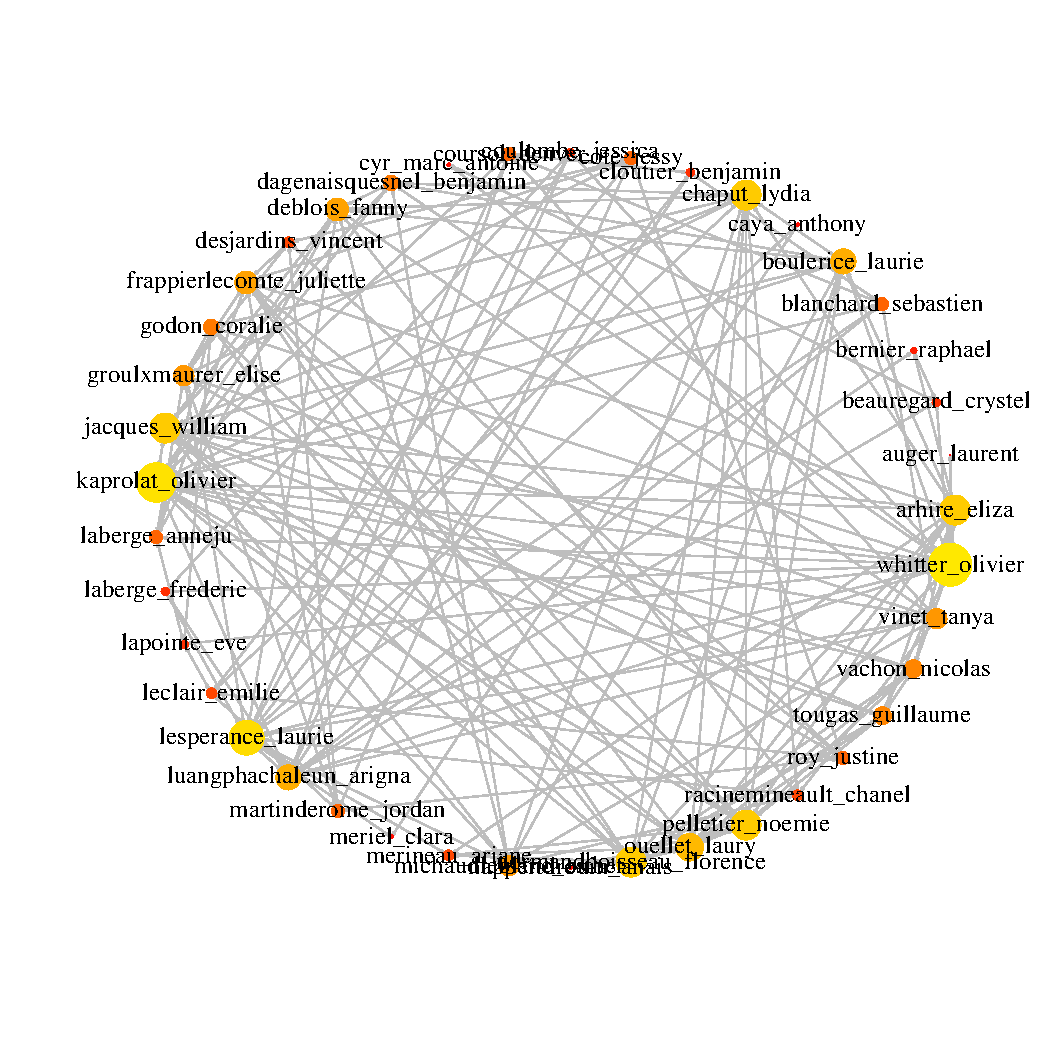
\includegraphics[scale=0.47]{Figure1_reseau.pdf}
\caption{Réseau de collaborations entre les étudiants de BIO500 de la session hiver 2021}
   \label{fig1}
      \end{figure}
Depuis le début leur bac, les étudiants du cours BIO500-H21 ont pu agrandir leur cercle de connaissance et ainsi se construire un réseau.Dans la figure 1, Olivier Whitter , Olivier Kaprolat, Noémie Pelletier et Laurie L’Espérance sont les élèves qui ont travaillé avec le plus grand nombre de personnes différentes durant leur bac. Ces quatre élèves du cours BIO500 ont donc créé dans le réseau plusieurs liens entre les étudiants. Dans la figure 1, Laurent Auger, Clara Meriel , Ariane Mérineau et Ève Lapointe sont ceux qui ont le moins de liens entre différents étudiants et contribuent peu à agrandir les connexions dans le réseau de cette étude.Un réseau écologique peut être facilement perturbés par le retrait d’espèces si ces derniers possèdent le plus de connections dans le réseau\cite{Sole2001}. Selon l’étude de Solé et Montoya, le retrait d’une proie qui est fortement interconnectée dans le réseau « foodwed » aurait un grand effet sur la stabilité de l’écosystème. Ainsi, l’extinction d’une espèce « Keystone » aurait comme conséquence d’affecter la communauté, autrement dit, d’augmenter ou de diminuer l’abondance de certaines espèces qui seraient directement liées à l’espèce retirée. Le réseau de notre étude agit de la même façon que le réseau écologique. En effet, le retrait d’un étudiant fortement connecté affecterait grandement les liens du réseau de connexion. Par exemple, le retrait de Olivier Whitter et Olivier Kaprolat aurait un grand impact sur les connections entre les étudiants du cours BIO500. De plus, le réseau serait composé de petits groupes d’étudiants ayant collaborés et dont les connections seraient plus limitées comparativement au réseau avec Olivier Whitter et Olivier Kaprolat.
\subsection{Histogramme des collaborateurs}
Dans la figure 2 , les deux valeurs dont un plus grand nombre d’étudiants ont collaborés avec personnes différentes durant le baccalauréat est cinq et quinze. La majorité des élèves ont travaillé avec moins de 16 étudiants. Ainsi, le nombre d’élèves qui a collaborés avec plus de quinze est relativement faible. Plus de 82 pourcent(32/39) se situe dans l’intervalle de 1 à 15 étudiants différents. Cela veut donc dire que seulement 18 pourcent ont travaillés avec plus de 15 étudiants différents.Les élèves de la classe BIO500 hiver2021 ont tendance à avoir peu de différents coéquipiers durant leur baccalauréat. 
\begin{figure}[H]
\centering
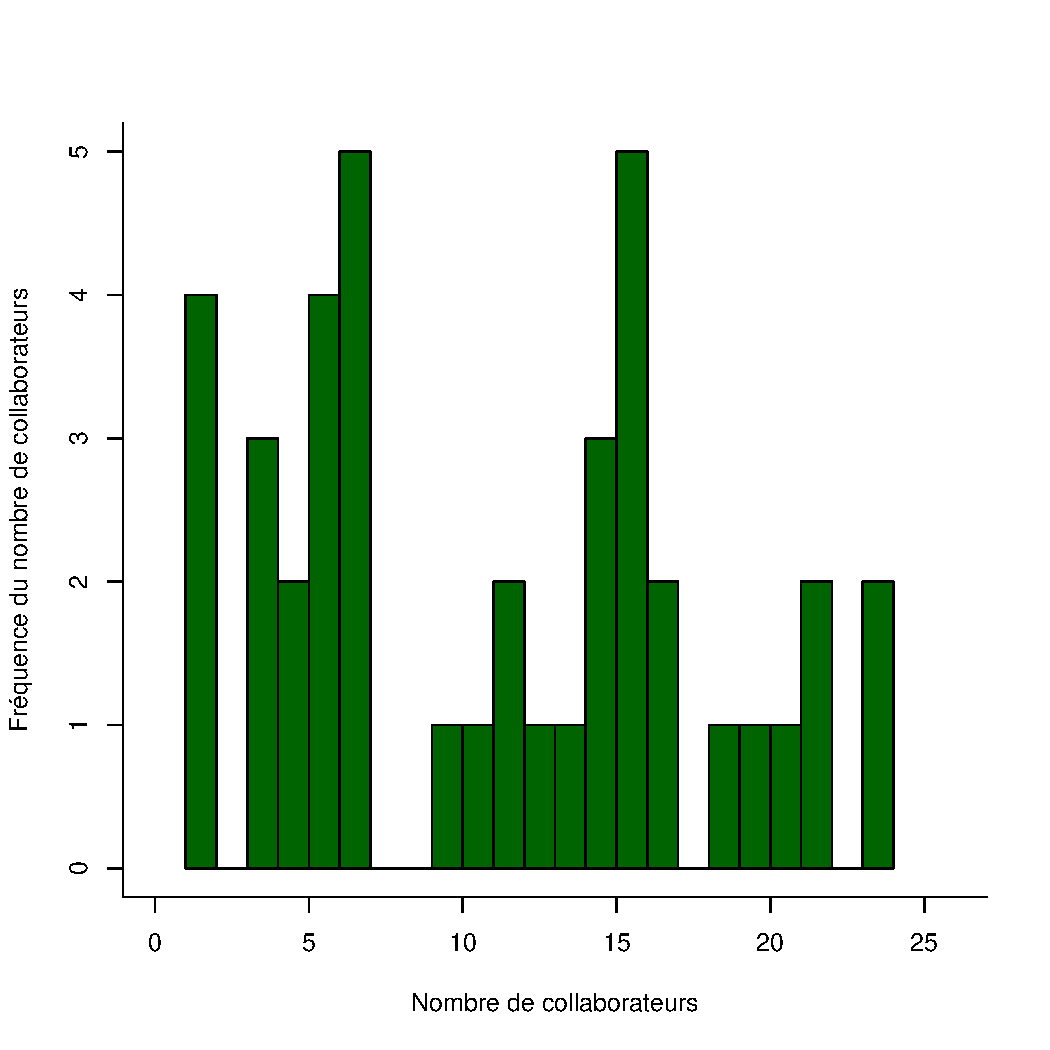
\includegraphics[scale=0.54]{Figure2_hist.pdf}
\caption{Fréquences du nombre de collaborateurs des étudiants du cours BIO500-H21 durant tout leur baccalauréat.}
\label{fig2}
\end{figure}
Les élèves de la classe BIO500-H21 ont tendances à avoir peu de coéquipiers différents durant leur baccalauréat. La majorité des élèves de ce cours ont collaborés avec moins de 16 personnes différentes. Ces résultats seraient expliqués par le fait que le travail de groupe peut amener plusieurs conflits et frustrations\cite{Boud1999}. Selon une étude fait par Burdett 2003\cite{Burdett2003}, les travaux d’équipes peuvent être stressant et amener de la compétition. Ainsi, les élèves auraient tendances à choisir des partenaires avec qui ils sont le plus compatibles et qui leur permet d’avoir de bonnes notes. Il serait donc possible de croire que les élèves de BIO500 ont travaillé avec peu de collaborateurs différents (< 15) pour éviter les difficultés que le travail d’équipe peu apporter. De plus, selon un sondage fait par Chang et Brickman (2018)\cite{Chang2018}, la contribution inégale de certaines personnes dans un travail d’équipe serait la cause première à vouloir travailler seule ou avec peu de personnes. 

\subsection{Diversité spécifique}
\begin{figure}[H]
\centering
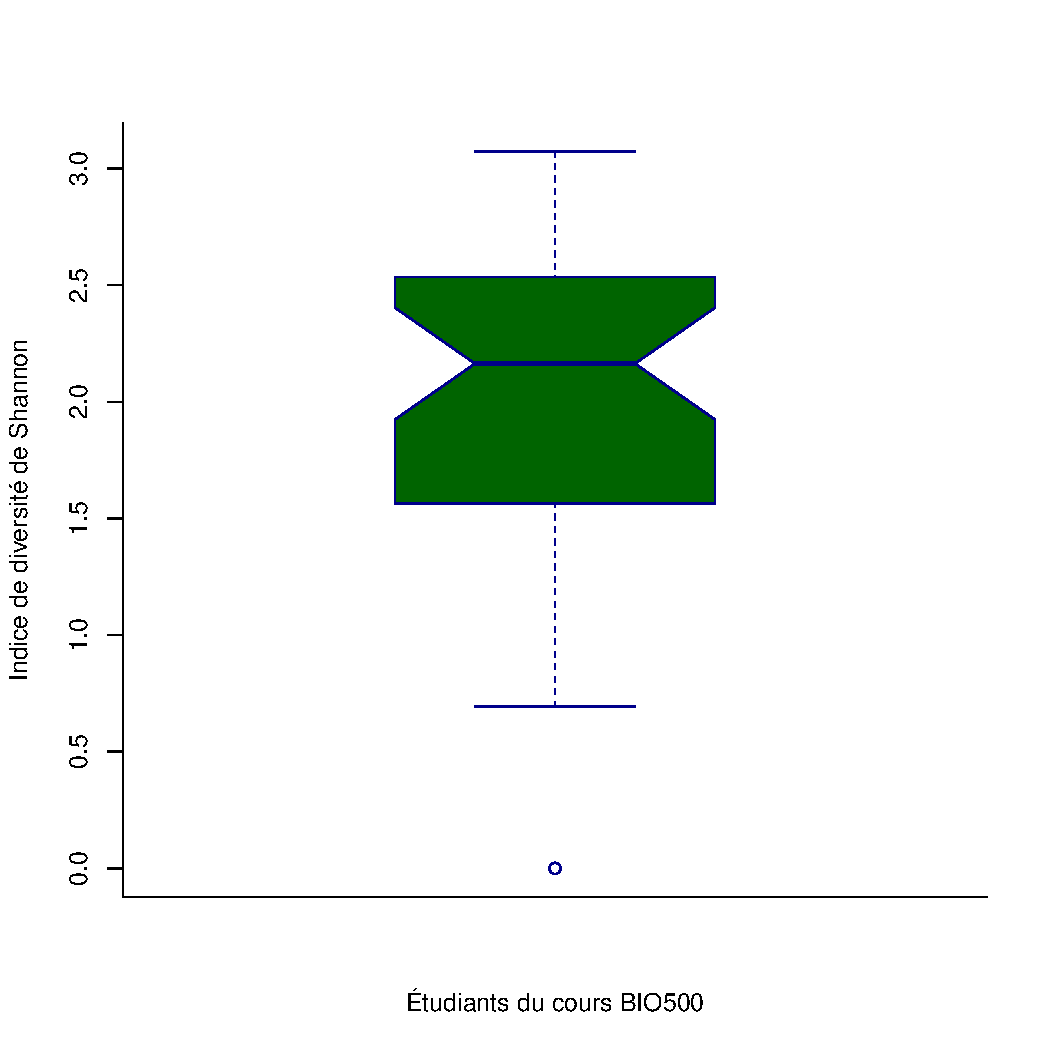
\includegraphics[scale=0.52]{Figure3_shannon.pdf}
 \caption{Diversités spécifiques des collaborations chez les étudiants du cours BIO500-H21 durant tout leur baccalauréat.}
 \label{fig3}
\end{figure}
La figure 3 montre que la diversité spécifique des collaborations des étudiants varie entre 0.69 et 3.07. La valeur du premier quartile est de 1.56, tandis que celle du troisième quartile est 2.54. Finalement, la médiane est de 2.16. Il est possible d’observer que les étudiants de la moitié supérieure sont distribués dans un plus petit intervalle de valeurs que la moitié inférieure. Ainsi, la diversité spécifique des étudiants tend vers des valeurs relativement élevées. Cependant, il est presque impossible de connaître la valeur théorique maximale de diversité spécifique, car le nombre maximum de collaborateurs par étudiant dépend largement des cours et du parcours de chacun. Toutefois, il est d’usage d’utiliser le nombre total d’espèces (collaborateurs) de l’échantillon pour calculer cette valeur\cite{REBENT}. Ainsi, il est possible d’obtenir une valeur maximale en supposant que les étudiants du cours collaborent uniquement entre eux. Puisqu’il y a 41 étudiants dans le cours BIO500, la diversité spécifique maximale serait d’environ 3.69, qui est calculée en faisant le logarithme naturel de 40. Étant donné l’absence d’indice d’équitabilité pour accompagner les indices de diversité, les analyses et conclusions qui peuvent être réalisés sont relativement faibles\cite{REBENT}. 

\end{multicols}
\subsection{Collaborateurs par session}
 \begin{table}[H]
 \centering
 \caption{Nombre de collaborateurs par étudiant du cours BIO500-H21 au fil des sessions du baccalauréat en écologie.\\} 
\begin{tabular}{|ccccccccc|c|}
\hline
& A18 & H19 & E19& A19 & H20 & E20 & A20 & H21 & \textbf{Moyennes} \\ 
\hline\hline 
arhire\_eliza & 0 & 14 & 0 & 4 & 0 & 3 & 0 & 4 & 3 \\ 
  auger\_laurent & 0 & 0 & 0 & 0 & 0 & 0 & 0 & 1 & 0 \\ 
  beauregard\_crystel & 0 & 3 & 0 & 0 & 2 & 2 & 0 & 0 & 1 \\ 
  bernier\_raphael & 0 & 3 & 0 & 0 & 0 & 0 & 0 & 1 & 0 \\ 
  blanchard\_sebastien & 0 & 0 & 0 & 4 & 0 & 2 & 4 & 0 & 1 \\ 
  boulerice\_laurie & 0 & 9 & 0 & 0 & 0 & 0 & 0 & 6 & 2 \\ 
  caya\_anthony & 0 & 0 & 0 & 2 & 0 & 0 & 0 & 0 & 0 \\ 
  chaput\_lydia & 0 & 11 & 0 & 5 & 0 & 4 & 0 & 8 & 4 \\ 
  cloutier\_benjamin & 0 & 0 & 0 & 4 & 0 & 0 & 0 & 0 & 0 \\ 
  cote\_jessy & 3 & 4 & 0 & 4 & 0 & 2 & 0 & 3 & 2 \\ 
  coulombe\_jessica & 0 & 1 & 0 & 8 & 4 & 2 & 6 & 5 & 3 \\ 
  coursol\_denver & 0 & 0 & 0 & 4 & 0 & 0 & 4 & 0 & 1 \\ 
  cyr\_marc\_antoine & 0 & 0 & 0 & 0 & 2 & 0 & 0 & 0 & 0 \\ 
  dagenaisquesnel\_benjamin & 0 & 0 & 0 & 2 & 0 & 0 & 0 & 6 & 1 \\ 
  deblois\_fanny & 0 & 11 & 0 & 4 & 0 & 5 & 0 & 8 & 4 \\ 
  desjardins\_vincent & 2 & 2 & 0 & 5 & 0 & 2 & 0 & 1 & 2 \\ 
  frappierlecomte\_juliette & 3 & 8 & 0 & 5 & 0 & 3 & 0 & 3 & 3 \\ 
  godon\_coralie & 0 & 10 & 0 & 0 & 0 & 0 & 0 & 1 & 1 \\ 
  groulxmaurer\_elise & 3 & 9 & 1 & 4 & 1 & 1 & 0 & 4 & 3 \\ 
  jacques\_william & 0 & 9 & 0 & 4 & 0 & 3 & 0 & 7 & 3 \\ 
  kaprolat\_olivier & 0 & 7 & 0 & 5 & 0 & 1 & 4 & 7 & 3 \\ 
  laberge\_anneju & 0 & 6 & 0 & 0 & 0 & 0 & 0 & 0 & 1 \\ 
  laberge\_frederic & 0 & 0 & 0 & 0 & 4 & 0 & 3 & 11 & 2 \\ 
  lapointe\_eve & 0 & 3 & 0 & 0 & 1 & 0 & 0 & 0 & 0 \\ 
  leclair\_emilie & 0 & 0 & 0 & 4 & 12 & 0 & 5 & 4 & 3 \\ 
  lesperance\_laurie & 0 & 10 & 1 & 6 & 0 & 4 & 0 & 5 & 3 \\ 
  luangphachaleun\_arigna & 0 & 11 & 0 & 7 & 0 & 5 & 4 & 4 & 4 \\ 
  martinderome\_jordan & 3 & 4 & 0 & 4 & 0 & 2 & 0 & 4 & 2 \\ 
  meriel\_clara & 0 & 0 & 0 & 2 & 0 & 0 & 0 & 0 & 0 \\ 
  merineau\_ariane & 0 & 4 & 0 & 0 & 0 & 0 & 0 & 1 & 1 \\ 
  michaudleblanc\_esther & 0 & 11 & 0 & 4 & 0 & 4 & 0 & 8 & 3 \\ 
  nappertdrouin\_anais & 0 & 5 & 0 & 0 & 0 & 0 & 0 & 0 & 1 \\ 
  normandboisseau\_florence & 0 & 15 & 0 & 4 & 0 & 1 & 0 & 4 & 3 \\ 
  ouellet\_laury & 0 & 14 & 0 & 4 & 0 & 3 & 0 & 4 & 3 \\ 
  pelletier\_noemie & 0 & 15 & 0 & 4 & 0 & 1 & 0 & 3 & 3 \\ 
  racinemineault\_chanel & 0 & 10 & 0 & 4 & 0 & 3 & 0 & 4 & 3 \\ 
  roy\_justine & 3 & 4 & 0 & 4 & 0 & 1 & 0 & 5 & 2 \\ 
  tougas\_guillaume & 0 & 9 & 0 & 4 & 0 & 4 & 0 & 0 & 2 \\ 
  vachon\_nicolas & 0 & 9 & 0 & 4 & 0 & 3 & 0 & 0 & 2 \\ 
  vinet\_tanya & 0 & 12 & 0 & 0 & 1 & 0 & 4 & 0 & 2 \\ 
  whitter\_olivier & 0 & 14 & 0 & 8 & 2 & 3 & 0 & 7 & 4 \\ 
  \hline
 \textbf{Moyennes} & 0 & 6 & 0 & 3 & 1 & 2 & 1 & 3 & 2 \\ 
   \hline
\end{tabular}
\end{table}
\clearpage
\begin{multicols}{2}
Dans le tableau ci-dessus, il est possible de remarquer que seulement six étudiants ont eu l’opportunité de collaborer avec d’autres étudiants lors de la première session du bac, soit à l’automne 2018. On peut supposer que ces 6 étudiants ont été amenés à travailler ensemble sur différents travaux en raison de leur parcours similaire qui découle d’une technique en bioécologie. En effet, les cours suivis par ces techniciens ne correspondaient pas au parcours traditionnel des autres étudiants du baccalauréat. Cela a probablement favorisé la collaboration entre ces six étudiants. Pour la deuxième session (H19), l’étudiant ayant eu le plus grand nombre de collaborateurs est Florence Normand-Boisseau avec un total de 15 collaborateurs. Il est également possible de noter que la session qui a eu lieu à l’hiver 2019 présente la moyenne de collaborateurs la plus importante comparativement aux autres sessions. Cela pourrait entre autres s’expliquer par le fait que les étudiants ont appris à se connaître au cours de la première session et ont tenté de travailler ensemble par la suite. Ensuite, à l’été 2019, seulement Élise Groulx-Maurer et Laurie L’Espérance ont été amenées à collaborer. L’ensemble des étudiants faisant partie du programme coopératif étaient en stage à ce moment. Par conséquent, ces deux étudiantes ont effectué un stage ensemble pendant cette période estivale. Concernant l’automne 2019, Jessica Coulombe et Olivier Whitter ont collaboré avec huit personnes distinctes, ce qui représente le nombre de collaborateurs le plus volumineux. Le second hiver, on s’aperçoit rapidement qu’Émilie Leclair a eu douze collaborateurs, ce qui est largement supérieur aux autres étudiants dont la moyenne est d’un seul collaborateur. Étant donné son parcours particulier, Émilie a suivi l’ensemble des cours que la majorité des étudiants ont suivi l’hiver précédent à l’hiver 2020. De façon générale, les sessions d’hiver comportent plus de cours que les autres sessions. C’est pourquoi les sessions hivernales ont généralement des moyennes élevées. Pour finir, la moyenne de collaborateurs différents la plus élevée au fil des sessions est de quatre seulement. Des liens serrés entre les étudiants pourraient expliquer cette moyenne. 
\end{multicols}
\clearpage
\bibliographystyle{plain}
\bibliography{biblio}

\end{document}
